\documentclass{article}

% Language setting
% Replace `english' with e.g. `spanish' to change the document language
\usepackage[english]{babel}

% Set page size and margins
% Replace `letterpaper' with `a4paper' for UK/EU standard size
\usepackage[a4paper,top=2cm,bottom=2cm,left=3cm,right=3cm,marginparwidth=1.75cm]{geometry}

% Useful packages
\usepackage{amsmath}
\usepackage[utf8]{inputenc}
\usepackage{titling}
\newcommand{\subtitle}[1]{%
  \posttitle{%
    \par\end{center}
    \begin{center}\large#1\end{center}
    \vskip0.5em}%
}
\usepackage{graphicx}
\usepackage[inkscapelatex=false]{svg}
\usepackage[colorlinks=true, allcolors=blue]{hyperref}
\usepackage{tocloft} % For customizing the TOC
\usepackage{booktabs}
\usepackage{multirow}
\usepackage{utf8}{inputenc}

% to display the code
\usepackage{listings}
\usepackage{xcolor}
\lstdefinestyle{python}{
    language=Python,
    basicstyle=\ttfamily\small,
    keywordstyle=\color{blue}\bfseries,
    stringstyle=\color{red},
    commentstyle=\color{gray}\itshape,
    numbers=left,
    numberstyle=\tiny\color{gray},
    stepnumber=1,
    numbersep=8pt,
    showstringspaces=false,
    frame=single,
    breaklines=true,
    tabsize=4,
    backgroundcolor=\color{gray!10},
}
\lstset{style=python}

% to display the graphs
\usepackage{tikz}
\usepackage{pgfplots}
\pgfplotsset{compat=1.18}


\title{\textbf{Lunar Lander}}
\subtitle{Project \#2 for Artificial Intelligence Fundamentals}

\author{Francisco Silva, Miguel Pereira and Guilherme Rodrigues 
\\ Nº 2022213583, 2022232552 and 2022232102 \\ \\
Department of Informatics Engineering \\
University of Coimbra, Coimbra, Portugal
\\ \textbf{\{francisco.lapamsilva,miguelmpereira0409,gfr04\}}@gmail.com}

\date{May 18th, 2025}

\begin{document}

\maketitle

\newpage
\tableofcontents
\newpage

\section{Methodology}
\subsection{Perceptions}
We utilize the following perception variables to determine the lander's state:

\begin{table}[h]
\centering
\begin{tabular}{@{}ll@{}}
\toprule
\textbf{Symbol} & \textbf{Description} \\
\midrule
x & Horizontal position (0 at platform center) \\
y & Vertical position (0 at platform surface) \\
Vx & Horizontal velocity (positive rightward) \\
Vy & Vertical velocity (positive upward) \\
A & Angular direction (positive counter-clockwise) \\
Va & Angular velocity (positive counter-clockwise) \\
L & Left leg ground contact (1 if touching) \\
R & Right leg ground contact (1 if touching) \\
\bottomrule
\end{tabular}
\caption{Perception Variables and Descriptions}
\end{table}

\subsection{Actions}
To control the it's descent, the Lander uses two motors: main motor (mM) and lateral motors (lM), whose values range from 0.0$\rightarrow$1.0 and -1.0$\rightarrow$1.0.
These two controls are represented and controlled by the two output neurons, as seen in the "network" function.
When the mM's value is greater than 0.5, the motor is on. When the lM's value is lesser than -0.5, the left motor activates, and when it is greater than 0.5, the right motor activates.
\begin{table}[h]
\centering
\begin{tabular}{@{}ll@{}}
\toprule
\textbf{Symbol} & \textbf{Description} \\
\midrule
mM & main Motor \\
lM & lateral Motor \\
\bottomrule
\end{tabular}
\caption{Perception Variables and Descriptions}
\end{table}

\subsection{Objective Function}
The most important mechanism of our evolution is the Objective Function. It is also the part that has undergone the biggest change throughout development.
Our Objective Function is designed to evaluate the lander and guide it to a successful landing by rewarding stability, position, and landing.

We started with the simple goal of stabilizing the lander. The first version of the OF looks like this:
\begin{lstlisting}
def objective_function(observation):
    fitness = 0

    x = observation[0]
    y = observation[1]
    x_speed = observation[2]
    y_speed = observation[3]
    angle = observation[4]
    angle_speed = observation[5]
    left_leg_touching = observation[6]
    right_leg_touching = observation[7]

    #stability
    stable_angle = (25-(angle)**2) / 25
    stable_angle_speed = int(abs(angle_speed) < 1.5)

    stable_horizontal_speed = int(abs(x_speed) < 0.1)   # Neste caso é melhor discreto
    stable_vertical_speed = (10-(y_speed+0.2)**2) / 10  # Offset de -0.2 (velocidade desejada de -0.2)

    stability = (
        500* stable_angle +
        400* stable_angle_speed +
        200* stable_horizontal_speed +
        300* stable_vertical_speed
    )



    fitness = (
        stability
    )

    return fitness, check_successful_landing(observation)
\end{lstlisting}

Some noteworthy aspects of this code are our early decision to make each rule return values normalized between 0 and 1 that are then multiplied by a weight to balance the importance of different rules, and the utilization of constant functions instead of discrete, to better guide the lander to the desirable state smoothly.

\begin{figure}[h]
    \centering
    % Top-left: stable_angle
    \begin{minipage}{0.48\textwidth}
        \centering
        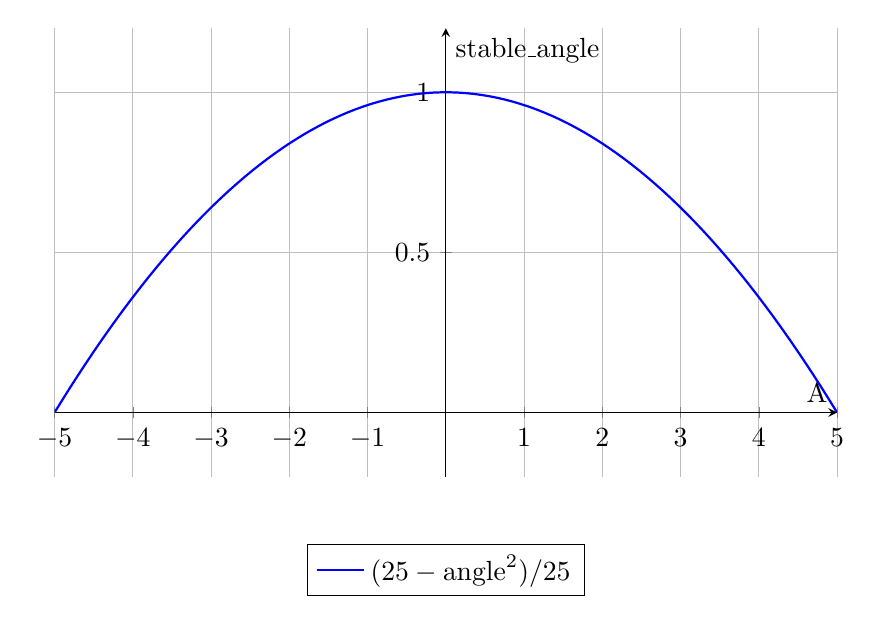
\begin{tikzpicture}
            \begin{axis}[
                domain=-5:5,
                samples=100,
                axis lines=middle,
                xlabel={A},
                ylabel={stable\_angle},
                width=0.95\textwidth,
                height=0.6\textwidth,
                ymin=-0.2, ymax=1.2,
                xmin=-5, xmax=5,
                grid=both,
                legend style={at={(0.5,-0.15)},anchor=north},
            ]
            \addplot[blue, thick] {(25 - (x)^2)/25};
            \addlegendentry{$(25-\mathrm{angle}^2)/25$}
            \end{axis}
        \end{tikzpicture}
        \caption{stable\_angle}
    \end{minipage}
    \hfill
    % Top-right: stable_angle_speed
    \begin{minipage}{0.48\textwidth}
        \centering
        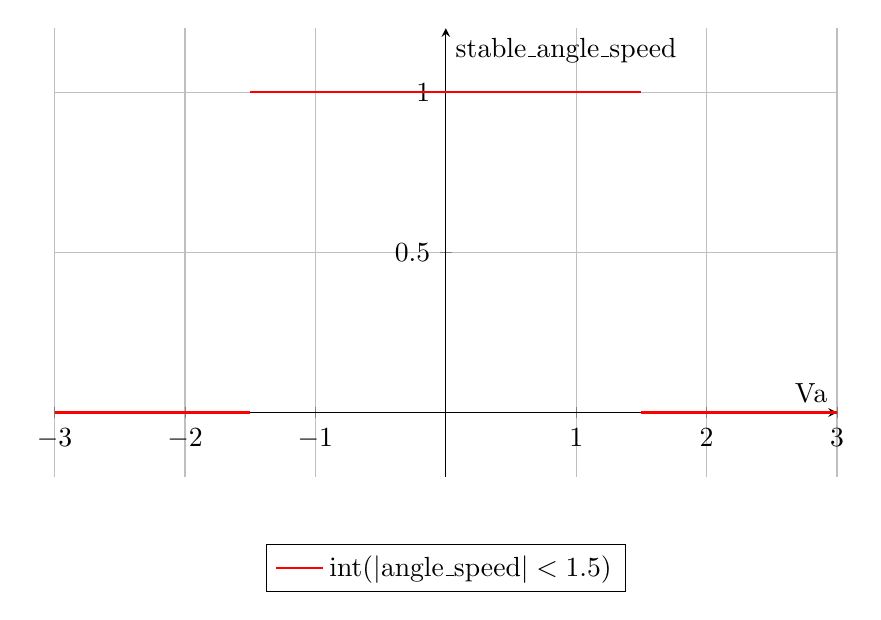
\begin{tikzpicture}
            \begin{axis}[
                domain=-3:3,
                samples=100,
                axis lines=middle,
                xlabel={Va},
                ylabel={stable\_angle\_speed},
                width=0.95\textwidth,
                height=0.6\textwidth,
                ymin=-0.2, ymax=1.2,
                xmin=-3, xmax=3,
                grid=both,
                legend style={at={(0.5,-0.15)},anchor=north},
            ]
            \addplot[red, thick, samples=2, domain=-3:-1.5] {0};
            \addplot[red, thick, samples=2, domain=-1.5:1.5] {1};
            \addplot[red, thick, samples=2, domain=1.5:3] {0};
            \addlegendentry{$\mathrm{int}(|\mathrm{angle\_speed}| < 1.5)$}
            \end{axis}
        \end{tikzpicture}
        \caption{stable\_angle\_speed}
    \end{minipage}
    \vspace{1em}

    % Bottom-left: stable_horizontal_speed
    \begin{minipage}{0.48\textwidth}
        \centering
        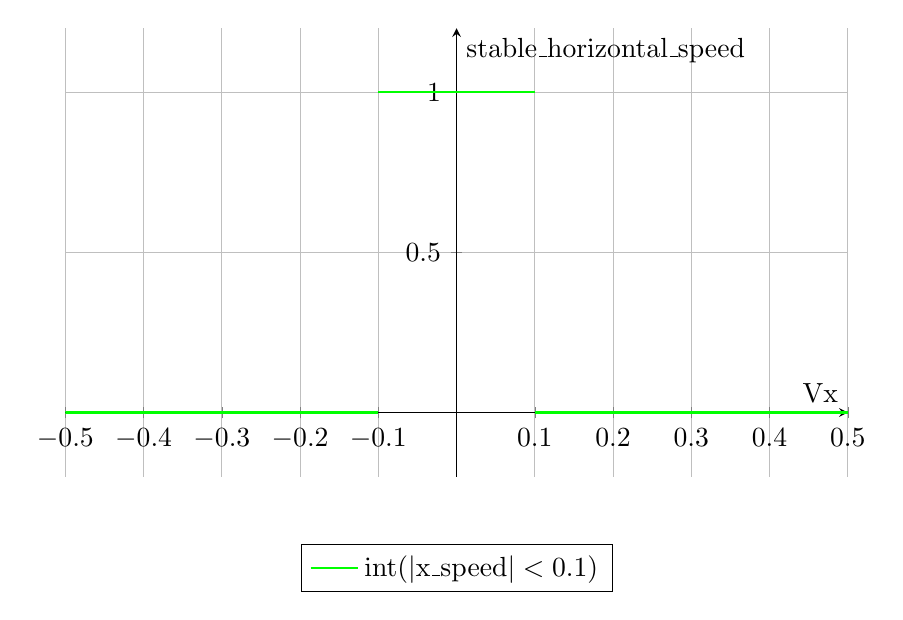
\begin{tikzpicture}
            \begin{axis}[
                domain=-0.5:0.5,
                samples=2,
                axis lines=middle,
                xlabel={Vx},
                ylabel={stable\_horizontal\_speed},
                width=0.95\textwidth,
                height=0.6\textwidth,
                ymin=-0.2, ymax=1.2,
                xmin=-0.5, xmax=0.5,
                grid=both,
                legend style={at={(0.5,-0.15)},anchor=north},
            ]
            \addplot[green, thick, samples=2, domain=-0.5:-0.1] {0};
            \addplot[green, thick, samples=2, domain=-0.1:0.1] {1};
            \addplot[green, thick, samples=2, domain=0.1:0.5] {0};
            \addlegendentry{$\mathrm{int}(|\mathrm{x\_speed}| < 0.1)$}
            \end{axis}
        \end{tikzpicture}
        \caption{stable\_horizontal\_speed}
    \end{minipage}
    \hfill
    % Bottom-right: stable_vertical_speed
    \begin{minipage}{0.48\textwidth}
        \centering
        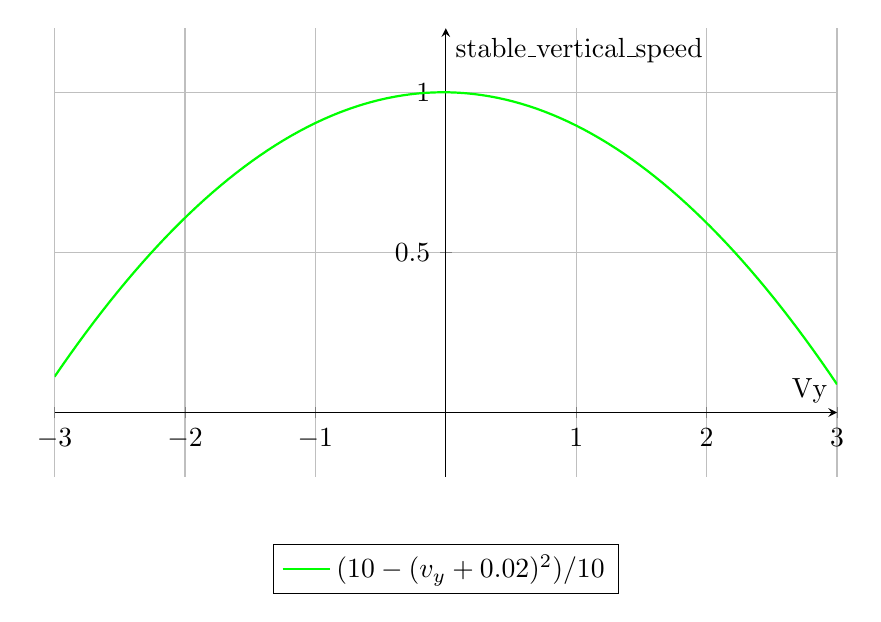
\begin{tikzpicture}
            \begin{axis}[
                domain=-3:3,
                samples=100,
                axis lines=middle,
                xlabel={Vy},
                ylabel={stable\_vertical\_speed},
                width=0.95\textwidth,
                height=0.6\textwidth,
                ymin=-0.2, ymax=1.2,
                xmin=-3, xmax=3,
                grid=both,
                legend style={at={(0.5,-0.15)},anchor=north},
                ]
                \addplot[green, thick] {(10 - (x + 0.02)^2)/10};
                \addlegendentry{$(10 - (v_y + 0.02)^2)/10$}
            \end{axis}
        \end{tikzpicture}
        \caption{stable\_vertical\_speed}
        \label{fig:stable_vertical_speed}
    \end{minipage}
\end{figure}

As shown in Figure~\ref{fig:stable_vertical_speed}, in the stable\_vertical\_speed function, we added a small offset of $-0.2$ to encourage the lander to descend at a speed of $-0.2$, which is the desired speed for landing. This adjustment helps prevent the lander from stopping completely or ascending.
This allows us to not have to add a separate rule to encourage the lander to descend, as it is already being done by the stable\_vertical\_speed function.

This version of the code generated a peak landing success rate of 24\%, but the evolution process is still very unreliable, and in some tests it remains 1\%. This is a problem that will only be resolved in the final version of the code.


Having the stability taken care of, we entered the phase of development. We added a metric to guide the positioning and landing. The code added looks like this:
\begin{lstlisting}
def objective_function(observation):
    fitness = 0

    # ------ existing observations ------- #

    # ---- existing stability rewards ---- #

    positioning_x_centered = (1-(x)**2) / 1
    positioning = (
        40* positioning_x_centered
    )


    # maximises fitness when both legs are touching, and x==0, using a quadratic function to center the lander
    landing = (
        50 * (int(left_leg_touching and right_leg_touching) * ((1-(x)**2)/1))
    )



    fitness = (
          stability
        + positioning
        + landing
    )

    return fitness, check_successful_landing(observation)
\end{lstlisting}

\begin{figure}[h]
    \centering
    % Left: positioning_x_centered
    \begin{minipage}{0.48\textwidth}
        \centering
        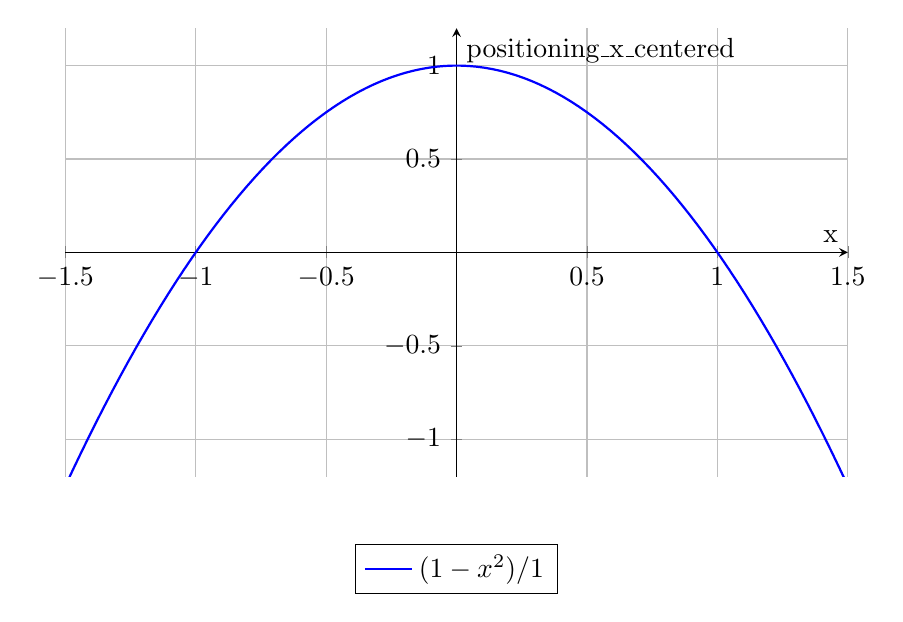
\begin{tikzpicture}
            \begin{axis}[
                domain=-1.5:1.5,
                samples=100,
                axis lines=middle,
                xlabel={x},
                ylabel={positioning\_x\_centered},
                width=0.95\textwidth,
                height=0.6\textwidth,
                ymin=-1.2, ymax=1.2,
                xmin=-1.5, xmax=1.5,
                grid=both,
                legend style={at={(0.5,-0.15)},anchor=north},
            ]
            \addplot[blue, thick] {(1 - (x)^2)/1};
            \addlegendentry{$(1-x^2)/1$}
            \end{axis}
        \end{tikzpicture}
        \caption{positioning\_x\_centered}
    \end{minipage}
    \hfill
    % Right: landing
    \begin{minipage}{0.48\textwidth}
        \centering
        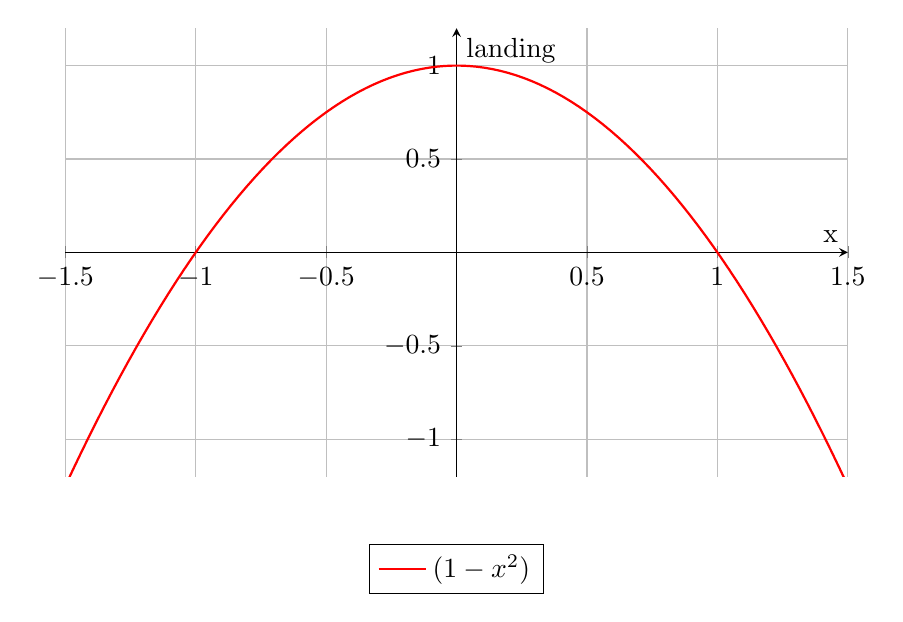
\begin{tikzpicture}
            \begin{axis}[
                domain=-1.5:1.5,
                samples=100,
                axis lines=middle,
                xlabel={x},
                ylabel={landing},
                width=0.95\textwidth,
                height=0.6\textwidth,
                ymin=-1.2, ymax=1.2,
                xmin=-1.5, xmax=1.5,
                grid=both,
                legend style={at={(0.5,-0.15)},anchor=north},
            ]
            \addplot[red, thick] {(1 - (x)^2)};
            \addlegendentry{$(1-x^2)$}
            \end{axis}
        \end{tikzpicture}
        \caption{landing (when both legs touch)}
    \end{minipage}
\end{figure}
This second version could achieve a maximum of 80\% success rate, but was also plagued by unreliability in the training process, and often resulted in agents that could not surpass 14\% success rate.


In the final stage of development, we tweaked the weights multiplied by each rule, in order to balance the importance of each rule.
To resolve the unreliability of the evolution, we decided then to tweak the mutation constants to make the agents try to explore more, and to not get stuck in local minima.
By increassing "STD\_DEV" from 0.1 to 0.5, we allow the agents to explore more agressively, which finally allows them to reliably reach a success rate of 99\% in only 100 generations.
We also increased the "EVALS" from 1 to 5, which makes the simulation take longer, but allows us to more accurately evaluate the fitness of each agent.
The final OF looks like this:
\begin{lstlisting}
    # ...
    STD_DEV = 0.5

    EVALS = 5
    # ...

    def objective_function(observation):
        fitness = 0

        x = observation[0]
        y = observation[1]

        x_speed = observation[2]
        y_speed = observation[3]

        angle = observation[4]
        angle_speed = observation[5]

        left_leg_touching = observation[6]
        right_leg_touching = observation[7]


        stable_angle = (25-(angle)**2) / 25
        stable_angle_speed = int(abs(angle_speed) < 1.5)
        stable_horizontal_speed = int(abs(x_speed) < 0.1)   # Neste caso e melhor discreto
        stable_vertical_speed = (10-(y_speed+0.01)**2) / 10  # Offset de -0.01 (velocidade desejada de -0.01)

        stability = (
            50* stable_angle +
            40* stable_angle_speed +
            40* stable_horizontal_speed +
            30* stable_vertical_speed
        )

        positioning_x_centered = (1-x**2) / 1
        positioning = (
            40* positioning_x_centered
        )

        landing = (
            50 * (int(left_leg_touching and right_leg_touching) * ((1-(x)**2)/1))
        )


        fitness = (
              stability
            + positioning
            + landing
        )

        return fitness, check_successful_landing(observation)

    # ...
\end{lstlisting}

Finally, this version reliably achieves a success rate of over 90\%, often reaching 99\%, demonstrating the necessity of increassing the mutation constants to allow the agents to explore more. Even with these simple rules, the lander is able to learn to land in a stable position.
Looking at the graph of the evolution of the fitness we see the lander quickly learns to land, in only 100 generations, reaching the maximum fitness of 300.0 in 72 generations.
\begin{figure}[h]
    \centering
    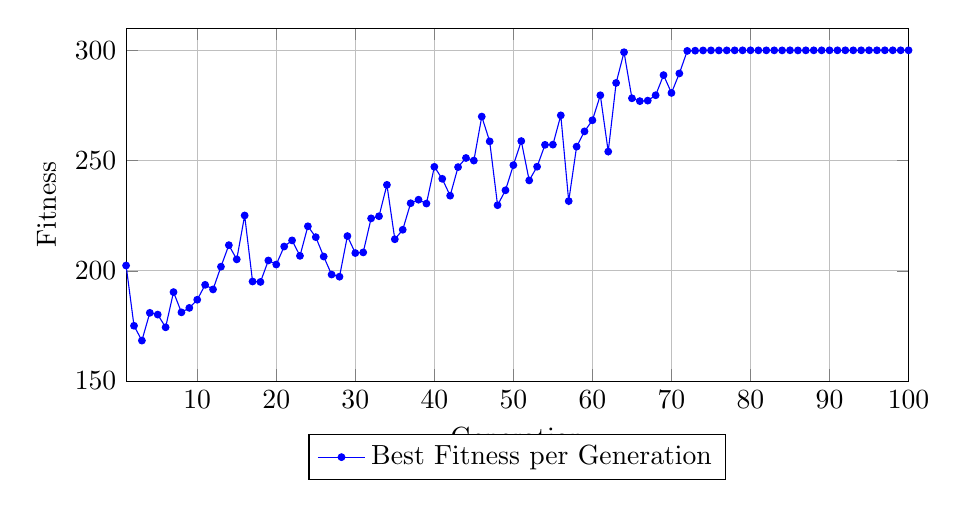
\begin{tikzpicture}
        \begin{axis}[
            width=0.95\textwidth,
            height=0.5\textwidth,
            xlabel={Generation},
            ylabel={Fitness},
            grid=both,
            ymin=150, ymax=310,
            xmin=1, xmax=100,
            legend style={at={(0.5,-0.15)},anchor=north},
        ]
        \addplot[
            color=blue,
            mark=*,
            mark size=1.2pt,
        ] coordinates {
            (1,202.40)
            (2,175.08)
            (3,168.36)
            (4,180.94)
            (5,180.15)
            (6,174.38)
            (7,190.35)
            (8,181.16)
            (9,183.18)
            (10,186.88)
            (11,193.64)
            (12,191.56)
            (13,201.87)
            (14,211.64)
            (15,205.19)
            (16,225.09)
            (17,195.15)
            (18,194.95)
            (19,204.69)
            (20,202.85)
            (21,211.01)
            (22,213.79)
            (23,206.78)
            (24,220.19)
            (25,215.26)
            (26,206.48)
            (27,198.31)
            (28,197.33)
            (29,215.75)
            (30,208.05)
            (31,208.35)
            (32,223.78)
            (33,224.75)
            (34,238.98)
            (35,214.31)
            (36,218.61)
            (37,230.65)
            (38,232.24)
            (39,230.49)
            (40,247.15)
            (41,241.72)
            (42,234.06)
            (43,247.02)
            (44,251.16)
            (45,249.98)
            (46,269.94)
            (47,258.70)
            (48,229.75)
            (49,236.51)
            (50,247.91)
            (51,258.83)
            (52,240.99)
            (53,247.21)
            (54,257.13)
            (55,257.21)
            (56,270.49)
            (57,231.62)
            (58,256.31)
            (59,263.22)
            (60,268.27)
            (61,279.61)
            (62,254.06)
            (63,285.19)
            (64,299.12)
            (65,278.23)
            (66,276.94)
            (67,277.17)
            (68,279.61)
            (69,288.74)
            (70,280.66)
            (71,289.50)
            (72,299.72)
            (73,299.82)
            (74,299.93)
            (75,299.95)
            (76,299.94)
            (77,299.95)
            (78,299.97)
            (79,299.97)
            (80,299.99)
            (81,299.96)
            (82,299.97)
            (83,299.97)
            (84,299.95)
            (85,299.99)
            (86,299.94)
            (87,299.97)
            (88,299.98)
            (89,299.97)
            (90,299.98)
            (91,299.98)
            (92,299.99)
            (93,299.98)
            (94,299.99)
            (95,300.00)
            (96,299.99)
            (97,299.99)
            (98,299.99)
            (99,299.99)
            (100,299.99)
        };
        \addlegendentry{Best Fitness per Generation}
        \end{axis}
    \end{tikzpicture}
    \caption{Evolution of fitness over generations.}
\end{figure}


\subsection{Genetic Operators}

\subsubsection{Parent Selection Methods}

Two different strategies for selecting parents were implemented and can be interchanged through the \texttt{PARENT\_SELECTION} variable.

\paragraph{Fitness-Proportionate Selection (Roulette Wheel)}
The \texttt{parent\_selection} function selects individuals with a probability proportional to their fitness. The total fitness of all positively fit individuals is calculated and a random probability is drawn. The algorithm iterates through the population, subtracting each individual's fitness contribution from the probability until one is selected. If the total positive fitness is zero or negative, a random individual is returned to avoid failure. This method ensures that individuals with higher fitness are more likely to be chosen while still giving a chance to less fit individuals.

\paragraph{Tournament Selection}
The \texttt{parent\_selection\_tournament} function implements a simple tournament selection: two individuals are randomly selected from the population, and the one with the highest fitness is chosen as the parent. This method introduces selective pressure by favoring the fitter of two candidates but without requiring any normalization of fitness values.

\paragraph{Current Strategy}
The evolutionary process currently uses the \texttt{tournament selection} strategy as the active method, set by:
\begin{verbatim}
PARENT_SELECTION = parent_selection_tournament
\end{verbatim}
This can be easily changed to the fitness-proportionate version if desired, providing flexibility to test different selection dynamics. We implemented and tested both approaches and observed that while tournament selection consistently yielded better results, the fitness-proportionate method also performed well in practice. For this reason, we decided to retain both implementations to allow further experimentation and adaptability in different scenarios.

\subsection{Crossover}
The \texttt{crossover} function is responsible for generating a new individual (offspring) from two parent individuals, using a single-point crossover method. This is a standard technique in genetic algorithms where a random point is chosen along the genotype vector, and the offspring inherits genes from one parent up to that point and from the other parent after that point.

The function starts by randomly selecting a crossover point between 1 and \texttt{GENOTYPE\_SIZE - 1}, ensuring that both parents contribute at least one gene to the offspring. Then, it randomly chooses which parent will contribute the first part and which one will contribute the second. This is done by generating a random number and comparing it with 0.5.

Depending on the order chosen, the function constructs the offspring's genotype by taking the first part from one parent and the second part from the other using list slicing. The result is a new genotype that is a mixture of the genetic material of both parents.

Finally, the function returns a new individual represented as a dictionary with the newly generated genotype and a \texttt{None} fitness value, indicating that the individual has not yet been evaluated.

This implementation introduces genetic diversity while preserving genetic information from the parents, which is essential for effective exploration of the solution space.

\subsection{Mutation}
The \texttt{mutation} function is responsible for introducing random genetic variation into an individual. This step is essential in genetic algorithms, as it helps maintain genetic diversity within the population and prevents premature convergence to suboptimal solutions.

The mutation process iterates through each gene in the individual's genotype. For each gene, a random number between 0 and 1 is generated and compared to a predefined mutation probability threshold, given by the constant \texttt{PROB\_MUTATION}. If the generated number is less than the threshold, the gene is mutated.

Mutation is applied by adding a random value to the gene, sampled from a Gaussian (normal) distribution with a mean of 0 and a standard deviation defined by the constant \texttt{STD\_DEV}. This method tends to introduce small perturbations, promoting a smoother and more controlled evolutionary process.

The final result is a new individual whose genotype has been slightly modified while maintaining its general structure. This operation enables the exploration of new regions in the solution space that would not be reached by crossover alone. Therefore, mutation plays a fundamental role in balancing exploration and exploitation in evolutionary algorithms.
\subsection{Survival Selection}
The \texttt{survival\_selection} function implements an elitist survival strategy. It starts by sorting the \texttt{offspring} list in descending order of fitness, ensuring the best individuals are at the front.

Then, the elite individuals from the current population (the top \texttt{ELITE\_SIZE} individuals) are re-evaluated using the \texttt{evaluate\_population} function. This accounts for potential changes in evaluation due to stochasticity in the fitness function.

These re-evaluated elite individuals are combined with the rest of the offspring (excluding the worst \texttt{ELITE\_SIZE} individuals) to form the new population.

Finally, the new population is sorted again by fitness in descending order, and returned. This ensures that the best individuals are preserved and that the population is always composed of the fittest available solutions.
\subsection{Evolution}
The \texttt{evolution} function encapsulates the entire evolutionary process. It begins by creating multiple parallel evaluation processes to improve efficiency during fitness computation.

Next an initial population is generated and evaluated. The best individual is stored to track the algorithm’s progress across generations.

For each generation, the algorithm generates offspring through either crossover (with probability \texttt{PROB\_CROSSOVER}) or direct parent copying. Parents are selected using the active selection strategy and all individuals are then mutated.

Once the offspring population reaches the predefined size, it is evaluated in parallel. After evaluation, the \texttt{survival\_selection} function is used to determine which individuals survive to the next generation, ensuring elitism is preserved.

The best individual of each generation is recorded alongside success rate and elapsed time for performance monitoring.

At the end of all generations, all evaluation processes are terminated, and the list of best individuals per generation is returned.

\subsection{Algorithm Parameters}
\begin{itemize}
    \item Population size: 100 individuals
    \item Generations: 100
    \item Crossover probability: 50\%
    \item Elite size: 1 individual
\end{itemize}

\section{Experimentation and Results}
\subsection{Milestone 1: Windless Environment}
Performance comparison of tested configurations:

\begin{table}[h]
\centering
\begin{tabular}{|l|c|c|c|c|c|}
\hline
\textbf{Experiência} & \textbf{Mutação} & \textbf{Crossover} & \textbf{Elitismo} & \textbf{Tamanho da População} & \textbf{Gerações} \\ 
\hline
1 & 0.008 & 0.5 & \multirow{4}{*}{0} & \multirow{8}{*}{100} & \multirow{8}{*}{100} \\ 
\cline{1-3}
2 & 0.05 & 0.5 & & & \\ 
\cline{1-3}
3 & 0.008 & 0.9 & & & \\ 
\cline{1-3}
4 & 0.05 & 0.9 & & & \\ 
\cline{1-4}
5 & 0.008 & 0.5 & \multirow{4}{*}{1} & & \\ 
\cline{1-3}
6 & 0.05 & 0.5 & & & \\ 
\cline{1-3}
7 & 0.008 & 0.9 & & & \\ 
\cline{1-3}
8 & 0.05 & 0.9 & & & \\ 
\hline
\end{tabular}

\caption{Configuration of the experiments for different parameters.}
\end{table}

% Table 4: Results
\begin{table}[h]
\centering

\begin{tabular}{|l|c|c|}
\hline
\textbf{Experiência} & \textbf{Hitrate} & \textbf{Score Médio} \\ \hline
1 & 15.4\% & 56653.992 \\ \hline
2 & 29.5\% & 74103.92 \\ \hline
3 & 18.3\% & 61151.43 \\ \hline
4 & 96.9\% & 146582.12 \\ \hline
5 & 14.3\% & 43808.66 \\ \hline
6 & 97.2\% & 148110.92 \\ \hline
7 & 17.0\% & 58213.836 \\ \hline
8 & 34.8\% & 82988.3 \\ \hline
\end{tabular}
\caption{Results of the experiments with different parameters.}
\end{table}

\subsection{Milestone 2: Windy Environment}
In order to adapt the algorithm to the windy environment, we made the stability rules weight more, something that is easy to do with the way we built the code:
\begin{lstlisting}
    def objective_function(observation):

        # ...

        stable_angle = (25-(angle)**2) / 25

        stable_angle_speed = int(abs(angle_speed) < 1.5)

        stable_horizontal_speed = int(abs(x_speed) < 0.1)   # Neste caso é melhor discreto

        stable_vertical_speed = (10-(y_speed+0.01)**2) / 10  # Offset de -0.01 (velocidade desejada de -0.01)

        stability = (

            50* stable_angle +

            40* stable_angle_speed +

            40* stable_horizontal_speed +

            30* stable_vertical_speed

        ) * 1 + (int(ENABLE_WIND) * 10)

        # ...

        fitness = (

              stability

            + positioning

            + landing

        )

        return fitness, check_successful_landing(observation)

    # ...


\end{lstlisting}


The way this weight is implemented, allows us to easily turn it on and off, and to adjust the weight of the wind penalty.


Even this trivial implementation allows us to achieve a success rate of 86\%, which is significantly better than the 24\% we achieved in the first version of the code.


\section{Conclusions}


We conclude that our approach on a neural network to land a lander on the moon was great although further improvements could be made to account for the presence of wind.


\subsection{Objective Function Design}

The sucess of the lander heavily depends on the objective functioon. Its careful tuning while balancing weights for stability, positioning, and landing were crucial.
Using continuous reward functions (e.g., quadratic penalties for angle and position) proved to be more effective than discrete thresholds in guiding the lander towards optimal behavior.

\subsection{Parent Selection}

Tournament selection outperformed fitness-proportionate selection in consistency. Retaining both methods allowed for flexibility, but tournament selection was more reliable for this problem.

\subsection{Wind Adaptation}
When introducing wind to the environment it required penalizing horizontal oscillations more agressively, showing the need for environment-specific reward shaping.

\end{document}
